\section{Introduction}
One of the most important and useful machine, when talking about electronics. Is the BLDC and PMAC (permanent magnet motor), reason being the highly versatile use in both household object and electrical transport. This report focuses on the controlling of a ME1117 Brush less Permanent Magnet Motor, for an electrical kart. \\

More precisely this project is a semester project, where SDU needs to replace the current motor driver of an electric gokart, with the groups own design. \\

The solution to this problem, is of course a piece of hardware neatly designed to meet the needs of the motor. With software being able to sense and control the hardware. Such a design has been illustrated by the supervisors, and given at the start of the project as seen in figure 1. \\

\begin{figure} [H]
  \centering
  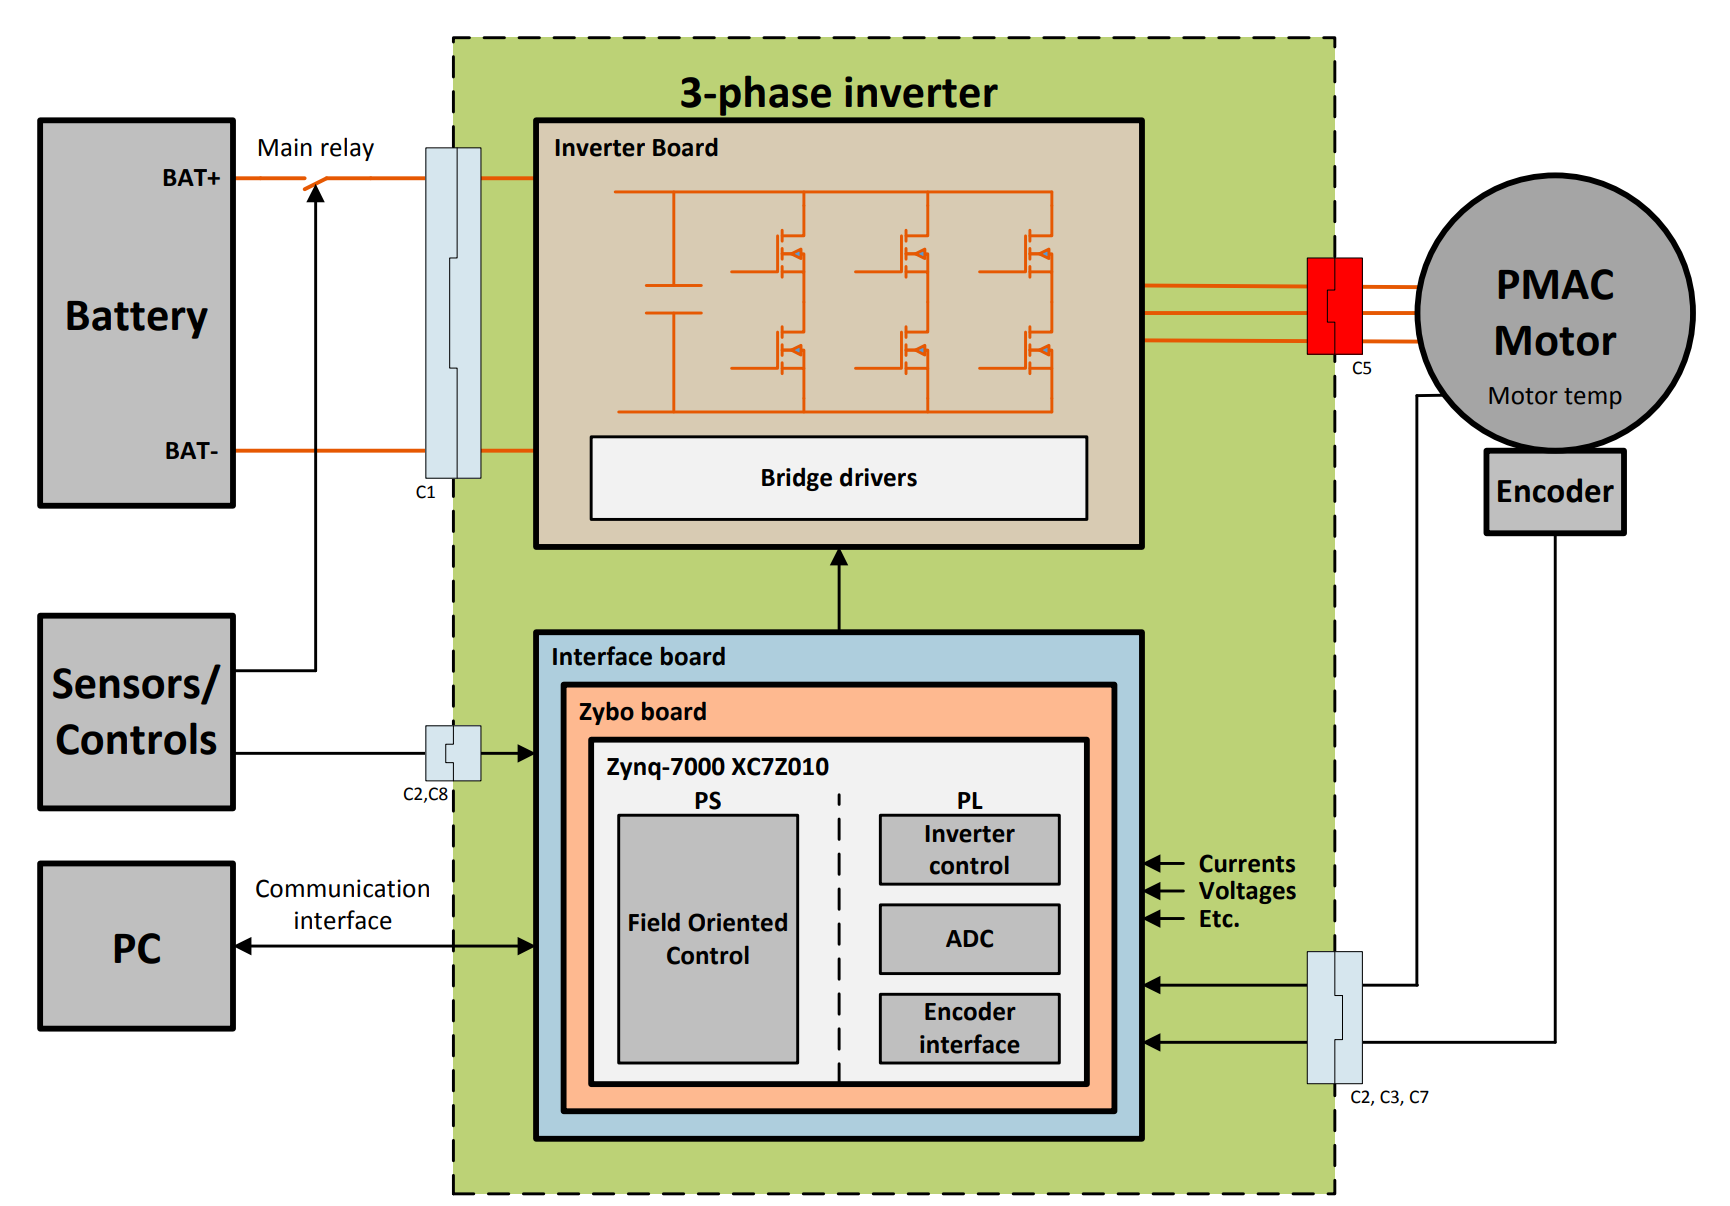
\includegraphics[width=\linewidth]{pictures/general/Project1.PNG}
  \caption{A suggestion to a possible solution given in the project description. \cite{Project 1. semester - S19}}
  \label{fig:Possiblesolution}
\end{figure}

The illustration above shows, a simplified version of how the main connections between elements should look. Where the green area show, where the design needs to take place. The hardware parts is in the 3-phase inverter and a small analog board, with the software being written on a Zybo board micro-controller. The interface board is a component all ready done, it is not designed but the group, but a tool for the communication between hardware and software.

\subsection{Requirements}

\textbf{Project requirement} \cite{Project 1. semester - S19}

\begin{itemize}
\item The solution must use a Zynq FPGA and a self‐designed 3‐phase inverter to control the PMAC motor.

\item It should be possible to set and get relevant parameters through a communication interface by a computer. Note: It is possible to use the UART interface on the Zybo board as communication interface.

\item It is not allowed to change any mechanical or electrical parts on the kart, except replacing the Sevcon gen4 controller. 
\end{itemize}